\chapter{Choices in Networks}
\label{ch:choicerank}

Understanding how users navigate in a network is of high interest in many applications.
In this chapter\footnote{%
This chapter is based on \citet{maystre2017choicerank}.
}, we consider a setting where only aggregate node-level traffic is observed and tackle the task of learning edge transition probabilities.
We cast it as a preference learning problem, and we study a model where choices follow Luce's axiom.
In this case, the $\BigO{n}$ marginal counts of node visits are a sufficient statistic for the $\BigO{n^2}$ transition probabilities.
We show how to make the inference problem well-posed regardless of the network's structure, and we present ChoiceRank, an iterative algorithm that scales to networks that contains billions of nodes and edges.
We apply the model to two clickstream datasets and show that it successfully recovers the transition probabilities using only the network structure and marginal (node-level) traffic data.
Finally, we also consider an application to mobility networks and apply the model to one year of rides on New York City's bicycle-sharing system.


%%%%%%%%%%%%%%%%%%%%%%%%%%%%%%%%
\section{Introduction}
\label{fi:sec:intro}

Markov chains have been used in recent work to aggregate inconsistent outcomes of pairwise comparisons and (partial) rankings \citep{dwork2001rank, negahban2012iterative, azari2013generalized}.
The idea is to build a Markov chain that is biased towards items that have won often, and to reduce the problem of ranking items to that of finding the \emph{stationary distribution} of the chain (the ranking is then induced by the items' stationary probabilities).
In this chapter, we highlight a connection between the MLE of models based on Luce's choice axiom and the stationary distribution of a Markov chain parametrized by the observed choices.
By formalizing this link, we unify previous algorithms and explicate them from an ML inference perspective.
Beyond this, the link suggests two new algorithms for parameter inference.
First, we develop a simple, consistent and computationally efficient spectral algorithm that is applicable to a wide range of models derived from Luce's choice axiom.
The exact formulation of the Markov chain used in the algorithm is distinct from related work \citep{negahban2012iterative, azari2013generalized} and achieves a significantly better statistical efficiency at no additional computational cost.
Second, we observe that with a small adjustment, the algorithm can be used iteratively, and it then converges to the MLE.
An evaluation on five real-world datasets reveals that it runs consistently faster than competing approaches and has a more predictable performance that does not depend on the structure of the data.
The key step, finding a stationary distribution, can be offloaded to commonly available linear-algebra primitives, which makes our algorithms  scale well.
The method we propose is intuitively pleasing, simple to understand and implement, and it outperforms the state of the art, hence we believe that it is highly useful to practitioners.

\paragraph{Outline of the Chapter}
We begin by introducing some notations and presenting a few useful facts about the MLE and about Markov chains.
In Section~\ref{fi:sec:relwork}, we discuss related work.
In Section~\ref{fi:sec:algorithms}, we present our algorithms, and in Section~\ref{fi:sec:experiments} we evaluate them on synthetic and real-world data.


\subsection{Maximum-Likelihood Estimate}
\label{fi:sec:mle}

%The log-likelihood \eqref{fi:eq:loglik} is not concave in $\bm{\gamma}$ (it can be made strictly concave using a simple reparametrization), but we briefly show in the supplementary material that it admits a unique stationary point, at the ML estimate $\bm{\gamma}^\star$.

Suppose that we collect $M$ independent choice observations in the multiset $\mathcal{D} = \{(c_m, \mathcal{A}_m) : m = 1, \ldots, M\}$.
Each observation consists of a choice $c_m$ among a set of alternatives $\mathcal{A}_m$;
we say that \emph{$i$ wins over $j$} and denote by $i \succ j$ whenever $i, j \in \mathcal{A}_m$ and $c_m = i$.
We postulate that the choices are generated from Luce's choice model, and for simplicity we denote the model parameter associated with item $c_m$ by $\gamma_m$.
From~\eqref{in:eq:luce}, it follows that the log-likelihood of parameters $\bm{\gamma}$ given observations $\mathcal{D}$ is given by
\begin{align}
\label{fi:eq:loglik}
\ell(\bm{\gamma}) = \sum_{m = 1}^M \bigg[ \log \gamma_m - \log{\sum_{j \in \mathcal{A}_m} \gamma_j} \bigg].
\end{align}
In order to ensure that the parameters are likelihood-identifiable, we assume without loss of generality that $\sum_i \gamma_i = 1$.
Next, we introduce a new object.

\begin{definition}[comparison graph]
The \emph{comparison graph} $\mathcal{G}_{\mathcal{D}} = (\mathcal{V}, \mathcal{E})$ is a directed graph with $\mathcal{V} = [N]$ and $(j, i) \in \mathcal{E}$ if and only if $i$ wins at least once over $j$ in $\mathcal{D}$.
\end{definition}

The existence and uniqueness of the MLE is completely determined by the connectivity of $\mathcal{G}_{\mathcal{D}}$, as the following well-known theorem shows.

\begin{theorem}[\citealp{zermelo1928berechnung, ford1957solution, hunter2004mm}]
\label{fi:thm:mlboth}
The likelihood function~\eqref{fi:eq:loglik} admits a unique maximizer $\bm{\gamma}^\star \in \mathbf{R}^N_{>0}$ such that $\sum_i \gamma^\star_i = 1$ if and only if $\mathcal{G}_{\mathcal{D}}$ is strongly connected.
\end{theorem}

Throughout this chapter, we will assume that $\mathcal{G}_{\mathcal{D}}$ is strongly connected.
In practice, if this assumption does not hold, we can consider each strongly-connected component separately.
Finally, note that even though $\ell(\bm{\gamma})$ admits a unique maximizer, it is not concave.
However, reparametrizing the model using $\theta_i \doteq \log \gamma_i$, the log-likelihood becomes
\begin{align*}
\ell(\bm{\theta}) = \sum_{m = 1}^M \bigg[ \theta_m - \log{\sum_{j \in \mathcal{A}_m} \exp \theta_j} \bigg],
\end{align*}
which is strictly concave in $\bm{\theta}$ (when $\mathcal{G}_{\mathcal{D}}$ is strongly connected).
Furthermore, for all $i \in [N]$,
\begin{align*}
\frac{\partial \ell}{\partial \gamma_i}
  = \frac{\partial \ell}{\partial \theta_i} \cdot \frac{\partial \theta_i}{\partial \gamma_i}
  = \frac{\partial \ell}{\partial \theta_i} \cdot \frac{1}{\gamma_i}
\quad \implies \quad
\frac{\partial \ell}{\partial \theta_i} = 0 \iff \frac{\partial \ell}{\partial \gamma_i} = 0.
\end{align*}
As the strictly concave function $\ell({\bm{\theta}})$ has a single stationary point, it follows that $\ell(\bm{\gamma})$ has a single stationary point at $\bm{\gamma}^\star$.


\subsection{Markov Chains}

We represent a finite, continuous-time Markov chain on $N$ states by a directed graph $\mathcal{G} = (\mathcal{V}, \mathcal{E})$, where $\mathcal{V} = [N]$ and $\mathcal{E}$ is the set of transitions with positive rate\footnote{%
Our exposition of Markov chains is succinct, and the interested reader is encouraged to consult \citet{levin2008markov} for a more thorough exposition.}.
If $\mathcal{G}$ is strongly connected, the Markov chain is said to be ergodic and admits a unique \emph{stationary distribution} $\bm{\pi} \in \mathbf{R}^N_{>0}$, $\sum_i \pi_i = 1$.
The \emph{global balance equations} relate the transition rates $\{ \lambda_{ij} \}$ to the stationary distribution as follows:
\begin{align}
\label{fi:eq:balance}
\sum_{j \ne i} \pi_i \lambda_{ij} = \sum_{j \ne i} \pi_j \lambda_{ji} \quad \forall i.
\end{align}
The stationary distribution is therefore invariant to changes in the time scale, i.e., to a rescaling of the transition rates.
Given transition rates $\bm{\Lambda} = [\lambda_{ij}]$, finding the stationary distribution $\bm{\pi}$ can be implemented in several different ways.
We distinguish implementations based on whether they consider a continuous-time or a discrete-time perspective on Markov chains.

\paragraph{Continuous-Time Perspective}
Let $\bm{Q}$ be the infinitesimal generator matrix of the Markov chain, i.e., $q_{ij} \doteq \lambda_{ij}$ and $q_{ii} \doteq - \sum_{j} \lambda_{ij}$.
The stationary distribution satisfies $\bm{\pi}^\Tr \bm{Q} = 0$; this is simply a matrix formulation of the global balance equations~\eqref{fi:eq:balance}.
Therefore, one approach to finding the steady-state distribution is to compute the rank-$1$ left nullspace of $\bm{Q}$.
This can be done, e.g., by LU decomposition, a basic linear-algebra primitive.
In the case where $\bm{Q}$ is dense, the running time of a typical implementation is $\BigO{N^3}$, but highly optimized parallel implementations such as that provided by LAPACK \citep{anderson1999lapack} are commonly available.
In the sparse case, LU decomposition can be done significantly faster using adapted algorithms, such as that of \citet{demmel1999supernodal}.

\paragraph{Discrete-Time Perspective}
Let $\epsilon < 1 / \max_i |q_{ii}|$, then $\bm{P} = \bm{I} + \epsilon \bm{Q}$ is the transition matrix of a discrete-time Markov chain that satisfies $\bm{\pi}^\Tr \bm{P} = \bm{\pi}$.
In this case, finding the steady-state distribution is equivalent to finding the left eigenvector associated to the leading eigenvalue of the transition matrix $\bm{P}$.
This is also a well-studied linear algebra problem for which plenty of efficient, off-the-shelf algorithms exist.
For example, power iteration methods can find the eigenvector in a few (sparse) matrix multiplications.
Beyond these well-known algorithms, recently-proposed randomized approaches such as that of \citet{halko2011finding} make it possible to scale to very large problem sizes ($N \sim 10^6$ or more).

Both the continuous-time and the discrete-time perspectives yield exactly the same resulting stationary distribution, and the algorithms presented in this paper are oblivious to this choice.

%%%%%%%%%%%%%%%%%%%%%%%%%%%%%%%%%%%%%%%%%%%%%%%%%%%%%%%%%%%%%%%%%%%%%%%%%
\section{Related Work}  %%%%%%%%%%%%%%%%%%%%%%%%%%%%%%%%%%%%%%%%%%%%%%%%%
\label{cr:sec:relwork}

A variant of the network choice model was recently introduced by \citet{kumar2015inverting}, in an article that lays much of the groundwork for this chapter.
Their generative model of traffic and the parametrization of transition probabilities based on Luce's axiom form the basis of our work.
\citeauthor{kumar2015inverting} define the \emph{steady-state inversion} problem as follows:
Given a graph $\mathcal{G}$ and a target stationary distribution, find transition probabilities that lead to the desired stationary distribution.
This problem formulation assumes that $\mathcal{G}$ satisfies restrictive structural properties (strong-connectedness, aperiodicity) and is valid only asymptotically, when the sequences of choices made by users are very long.
Our formulation is, in contrast, more general.
In particular, we eliminate any assumptions about the structure of $\mathcal{G}$ and cope with finite data in a principled way---in fact, our derivations are valid for choice sequences of any length.
One of our contributions is to explain the steady-state inversion problem in terms of (asymptotic) maximum-likelihood inference in the network choice model.
Furthermore, the statistical viewpoint that we develop also leads to
\begin{enuminline}
\item a robust regularization scheme, and
\item a simple and efficient EM-type inference algorithm.
\end{enuminline}
These important extensions make the model easier to apply to real-world data.

\paragraph{Luce's Choice Axiom}
The general problem of estimating parameters of models based on Luce's axiom has received considerable attention.
Several decades before Luce's seminal book \citep{luce1959individual}, \citet{zermelo1928berechnung} proposed a model and an algorithm that estimates the strengths of chess players based on pairwise comparison outcomes (his model would later be rediscovered by \citet{bradley1952rank}).
More recently, \citet{hunter2004mm} explained \citeauthor{zermelo1928berechnung}'s algorithm from the perspective of the minorization-maximization (MM) method.
This method is easily generalized to other models that are based on Luce's axiom, and it yields simple, provably convergent algorithms for maximum-likelihood (ML) or maximum-a-posteriori point estimates.
\citet{caron2012efficient} observe that these MM algorithms can be further recast as expectation-maximization (EM) algorithms by introducing suitable latent variables.
They use this observation to derive Gibbs samplers for a wide family of models.
We take advantage of this long line of work in Section~\ref{cr:sec:inference} when developing an inference algorithm for the network choice model.
In recent years, several authors have also analyzed the sample complexity of the ML estimate in Luce's choice model \citep{hajek2014minimax, vojnovic2016parameter} and investigated alternative spectral inference methods \citep{negahban2012iterative, azari2013generalized, maystre2015fast}.
Some of these results could be applied to our setting, but in general they require observing choices among well-identified sets of alternatives.
Finally, we note that models based on Luce's axiom have been successfully applied to problems ranging from ranking players based on game outcomes \citep{zermelo1928berechnung, elo1978rating} to understanding consumer behavior based on discrete choices \citep{mcfadden1973conditional}, and to discriminating among multiple classes based on the output of pairwise classifiers \citep{hastie1998classification}.

\paragraph{Network Analysis}
Understanding the preferences of users in networks is of significant interest in many domains.
For brevity, we focus on literature related to hyperlink graphs.
A method that has undoubtedly had a tremendous impact in this context is PageRank \citep{brin1998anatomy}.
PageRank computes a set of scores that are proportional to the amount of time a surfer, who clicks on links randomly and uniformly, spends at each node.
These scores are based only on the structure of the graph.
The network choice model presented in this chapter appears similar at first, but tackles a different problem.
In addition to the structure of the graph, it uses the traffic at each page, and computes a set of scores that reflect the (non-uniform) probability of clicking on each link.
Nevertheless, there are striking similarities in the implementation of the respective inference algorithms (see Section~\ref{cr:sec:experiments}).
The HOTness method proposed by \citet{tomlin2003new} is somewhat related, but tries to tackle a harder problem.
It attempts to estimate jointly the traffic and the probability of clicking on each link, by using a maximum-entropy approach.
At the other end of the spectrum, BrowseRank \citep{liu2008browserank} uses detailed data collected in users' browsers to improve on PageRank.
Our method uses only marginal traffic data that can be obtained without tracking users.
%In the context of mobility analysis, we mention that \citet{ashbrook2003using} and \citet{kafsi2015traveling}

%%%%%%%%%%%%%%%%%%%%%%%%%%%%%%%%%%%%%%%%%%%%%%%%%%%%%%%%%%%%%%%%%%%%%%%%%
\section{Theoretical Results}  %%%%%%%%%%%%%%%%%%%%%%%%%%%%%%%%%%%%%%%%%%
\label{rs:sec:theory}

In this section, we begin by studying the behavior and output of Quicksort under inconsistent comparison outcomes, without any assumptions on the noise generating process.
Then, starting in Section~\ref{rs:sec:poisson}, we focus on comparison outcomes generated by the BT model.
For clarity, longer proofs are deferred to Section~\ref{rs:sec:proofs}.

\begin{algorithm}[t]
   \caption{Quicksort.}
   \label{rs:alg:quicksort}
\begin{algorithmic}[1]
   \Require set of items $\mathcal{V} \subseteq [N]$
   \OneLineIf{$\Abs{\mathcal{V}} < 2$} \Return list($\mathcal{V}$)
   \Comment{Terminating case.}
   \State $\mathcal{L} \gets \varnothing, \mathcal{R} \gets \varnothing$
   \State $p \gets $ element of $\mathcal{V}$ selected uniformly at random \label{rs:line:pivot}
   \For{$i \in \mathcal{V} \setminus \{ p \}$} \label{rs:line:startpart}
     \If{$i \prec p$} \label{rs:line:comp}
     \Comment{Pairwise comparison.}
       \State $\mathcal{L} \gets \mathcal{L} \cup \{i\}$
     \Else
       \State $\mathcal{R} \gets \mathcal{R} \cup \{i\}$
     \EndIf
   \EndFor  \label{rs:line:stoppart}
   \State \Return $\text{Quicksort}(\mathcal{L}) \cdot p \cdot \text{Quicksort}(\mathcal{R})$ \label{rs:line:return}
\end{algorithmic}
\end{algorithm}

Quicksort (Algorithm~\ref{rs:alg:quicksort}) is best described as a recursive procedure.
At each step of the recursion, a \emph{pivot} item $p$ is chosen uniformly at random (line \ref{rs:line:pivot}).
Then, during the \emph{partition} operation (lines \ref{rs:line:startpart}--\ref{rs:line:stoppart}), every other item is compared to $p$ and added to the set $\mathcal{L}$ or $\mathcal{R}$, depending on the outcome of the comparison with the pivot.
If all comparison outcomes are consistent, it is well-known that Quicksort terminates after sampling \BigO{N \log N} comparisons with high probability.
What happens if we drop the consistency assumption?
The following two lemmas state that these key properties remain valid, no matter which (and how many) comparison outcomes are inconsistent.

\begin{lemma}
\label{rs:lem:termination}
Quicksort always terminates and samples each of the $N(N\!-\!1) / 2$ possible comparisons at most once.
\end{lemma}

\begin{proof}
The proof is identical to the consistent setting.
Consider the state of $\mathcal{L}$ and $\mathcal{R}$ at the end of a partition operation.
Because $\Abs{\mathcal{L}} + \Abs{\mathcal{R}} = \Abs{\mathcal{V}} - 1$, the recursive calls are made on sets of items of strictly decreasing cardinality, and the algorithm terminates after a finite number of steps.
Furthermore, suppose that Quicksort samples an outcome for the pair $(i, j)$.
Then either $i$ or $j$ is the pivot in a partition operation.
In either case, the pivot is not included in the recursive calls, which ensures that $(i, j)$ cannot be compared again.
\end{proof}

\begin{lemma}
\label{rs:lem:samplecomp}
%If the comparison outcomes are independent of the query order,
Quicksort samples \BigO{N \log N} comparisons with high probability.
\end{lemma}

\begin{proof}[Proof (sketch).]
We follow a standard analysis of Quicksort \citep[see, e.g.,][Section 3.3.3]{dubhashi2009concentration}.
With high probability, we choose a ``good'' pivot (i.e., one that results in a balanced partition) a constant fraction of the time.
In this case, the depth of the call tree is \BigO{\log N}.
As there are at most $N$ comparisons at each level of the call tree, we conclude that Quicksort uses \BigO{N \log N} comparisons in total.
With respect to the standard proof, ours requires additional work in order to formalize the notion of ``good'' pivot to the setting where comparison outcomes are not consistent with a linear order.
\end{proof}

Lemma~\ref{rs:lem:samplecomp} complements Theorem~$3$ in \citet{ailon2010preference}, which states that Quicksort samples \BigO{N \log N} in expectation.
These results might suggest that \emph{all} properties of Quicksort carry over to the noisy setting.
This is not the case.
For example, although Quicksort uses approximately $2N \ln N$ comparisons on average in the noiseless setting \citep{sedgewick2011algorithms}, this number can be distinctly different with inconsistent comparison outcomes\footnote{%
E.g., if comparison outcomes are uniformly random, all items are ``good'' pivots with high probability, and the average number of comparisons will be closer to $N \log_2 N$ on average, for large $N$.}.

Quicksort (and efficient sorting algorithms in general) infer most pairs of items' relative position by transitivity and rely heavily on the consistency of comparison outcomes.
In the noisy case, it is therefore important to precisely understand the effect of an inconsistent outcome on the output of the algorithm; this effect extends beyond the pair of items whose comparison outcome was inconsistent.
For this purpose, the next Lemma bounds the displacement of Quicksort's output as a function of the inconsistent outcomes.

\begin{lemma}
\label{rs:lem:dispbound}
Let $\mathcal{E}$ be the set of pairs sampled by Quicksort whose outcome is inconsistent with \Id.
Let $\sigma$ be the output of Quicksort.
Then,
\begin{align*}
\Disp{\sigma} \le 2 \sum_{\mathclap{(i, j) \in \mathcal{E}}}\; \Abs{i - j}
\end{align*}
\end{lemma}

\begin{proof}[Proof (sketch).]
Consider the first partition operation, with pivot $p$, resulting in partitions $\mathcal{L}$ and $\mathcal{R}$.
Denote the set of pairs of items involved in errors made during this partition operation by $\mathcal{E}_1$.
We can show that the displacement is bounded by
\begin{align*}
\Disp{\sigma} \le \Disp[\mathcal{L}]{\sigma} + \Disp[\mathcal{R}]{\sigma} + 2 \;\sum_{\mathclap{(i, j) \in \mathcal{E}_1}} \Abs{i - j},
\end{align*}
where \Disp[\mathcal{L}]{\sigma} and \Disp[\mathcal{R}]{\sigma} represent the displacement of the ordering induced by $\sigma$ on $\mathcal{L}$ and $\mathcal{R}$, respectively.
In other words, the total displacement can be decomposed into a term that represents the ``local'' displacement due to the partition operation and into two terms that account for errors in the recursive calls.
We obtain the desired result by recursively bounding \Disp[\mathcal{L}]{\sigma} and \Disp[\mathcal{R}]{\sigma}.
\end{proof}

Informally, Lemma~\ref{rs:lem:dispbound} states that the displacement can be bounded by a sum of ``local shifts'' due to the inconsistent outcomes and that the price to pay for any information inferred by transitivity is bounded by a factor two.
Lemma~\ref{rs:lem:dispbound} is a crucial component of our subsequent analysis of BT noise, and we believe that it can be useful in order to investigate Quicksort under a wide variety of other noise generating processes.


%%%%%%%%%%%%%%%%%%%%%%%%%%%%%%%%%%%%%%%%%%%%%%%%%%%%%%%%%%%%%%%%%%%%%%%%%
\subsection{Poisson-Distributed Parameters}
\label{rs:sec:poisson}

From here on, we assume that comparison outcomes are generated from $\BT(\bm{\theta})$.
Clearly, any results on the displacement of a ranking estimated from samples of a BT model will depend on $\bm{\theta}$; it is easy to construct a model instance for which it is arbitrarily hard to recover the ranking, by choosing parameters sufficiently close to each other.
Our approach is as follows.
We postulate a family of distributions over $\bm{\theta}$, and we give bounds on the displacement that hold with high probability.

We suppose that comparison outcomes are (in expectation) \emph{uniformly noisy across the ranking}: i.e., comparing two elements at the bottom is (a priori) as difficult as comparing two elements at the top or in the middle.
This means that the probability distribution over parameters $\theta_1, \ldots, \theta_N$ results in (random) distances $\Abs{\theta_{i+k} - \theta_i}$ that depend only on $k$.
One such distribution arises if the parameters are drawn from a Poisson point process of rate $\lambda$.
That is,
\begin{align}
\label{rs:eq:poisson}
\text{i.i.d.}\; x_1, \ldots, x_{N-1} \sim \DExp{\lambda}, \qquad
\theta_i = \sum_{n=1}^{i-1} x_n.
\end{align}
The average distance between two items separated by $k$ positions in the ordering is $\Exp{\theta_{i+k} - \theta_i} = k / \lambda$.
%More generally, the distance \Abs{\theta_{k+i} - \theta_i} has distribution $\DGamma{k, \lambda}$.
Although the distance between adjacent items is constant in expectation, we let some parameters be arbitrarily close\footnote{%
In particular, the expected minimum distance between two items (i.e., the $\min$ of $N$ exponential r.v.s) decreases as $(N\lambda)^{-1}$ as $N$ increases.}.
The parameter $\lambda$ indirectly controls the expected level of noise; a large $\lambda$ is likely to result in a larger number of inconsistent outcomes.
Although the precise choice of this Poisson model is driven by tractability concerns, in Section~\ref{rs:sec:iidunif} we argue that it is essentially equivalent to choosing the parameters independently and uniformly at random in the interval $[0, (N+1) / \lambda]$, when $\lambda$ is fixed and $N$ is large.
We are now ready to state our main result.

\begin{theorem}
\label{rs:thm:quickdisp}
Let $\bm{\theta}$ be sampled from a Poisson point process of rate $\lambda$.
Let $\sigma$ be the output of Quicksort using comparison outcomes sampled from $\BT(\bm{\theta})$.
Then,
\begin{align}
\Disp{\sigma}
    &= \BigO{ \lambda^2 N }, \label{rs:eq:qdtot} \\
\max_{i} \; \Abs{\sigma(i) - i}
    &= \BigO{ \lambda \log N }, \label{rs:eq:qdmax}
\end{align}
with high probability.
\end{theorem}

\begin{proof}[Proof (sketch)]
Let $z_{ij}$ be the indicator random variable of the event ``the comparison between $i$ and $j$ results in an error'', and let $d_{ij} = \Abs{\theta_i - \theta_j}$.
The distance $d_{ij}$ is a sum of $\Abs{i - j}$ i.i.d. exponential random variables, i.e., $d_{ij} \sim \DGamma{\Abs{i - j}, \lambda}$, and we can show that
\begin{align*}
\Exp{z_{ij}} &= \Exp{\frac{1}{1 + \exp(d_{ij})}}
    \le \Exp{\exp(-d_{ij})} = (1 + 1/\lambda)^{-\Abs{i - j}}.
\end{align*}
Using Lemma~\ref{rs:lem:dispbound} and the fact that every pair of items is compared at most once, we find
\begin{align*}
\Exp{\Delta}
    \le 2 \sum_{i < j}\; \Abs{i - j} \Exp{z_{ij}}
    \le 2N \sum_{k = 0}^{\infty} k (1 + 1/\lambda)^{-k} = 2N \lambda (\lambda + 1).
\end{align*}
The random variables $\{ z_{ij} \}$ are not independent (they are independent when conditioned on $\bm{\theta}$) but, with some more work, we can show that $\Var{\Delta} = \BigO{N}$.
By using a Chebyshev bound, \eqref{rs:eq:qdtot} follows.

In order to prove \eqref{rs:eq:qdmax}, we take advantage of a theorem due to \citet{ailon2008reconciling} which states that
\begin{align*}
\Prob{ \sigma(i) < \sigma(j) \mid \bm{\theta} } = \Prob{i \prec j \mid \bm{\theta}},
\end{align*}
even if $i$ and $j$ were not directly compared with each other.
We use a Chernoff bound on $d_{ij}$ to show that the relative order between any two items separated by at least $\BigO{\lambda \log N}$ positions is correct with high probability.
The second part of the claim follows easily.
\end{proof}

Note that any method that compares each pair of items at most once results in a ranking estimate $\tau$ with displacement $\Disp{\tau} = \BigOmega{N}$ with high probability: As there is only a single (possibly inconsistent) comparison outcome between each pair of adjacent items, it is likely that a constant fraction of the items will be ranked incorrectly, resulting in a displacement that grows linearly in $N$.
Hence, our bound on \Disp{\sigma} shows that Quicksort is order-optimal (in $N$).

In light of Theorem~\ref{rs:thm:quickdisp}, a natural question to ask is as follows.
How many comparisons are needed in order to find the correct ranking?
Finding the exact ranking is difficult: in fact, \BigOmega{N} comparison outcomes are necessary in order to discriminate the closest pair of items reliably, as we show next.
Suppose that we are given $K$ comparisons to find the relative order between $i$ and $j$, and define $e_{ij}$ as the event ``more than half of the $K$ comparison outcomes between $i$ and $j$ are inconsistent''.

\begin{proposition}
Let $\bm{\theta}$ be sampled from a Poisson point process of rate $\lambda$.
Then, there is a pair $i, j \in [N]$ and a constant $c > 0$ independent of $N$ such that if $K = \LittleO{\lambda N}$,
\begin{align*}
\Prob{e_{ij}} \ge c
\end{align*}
with high probability.
\end{proposition}

\begin{proof}
The distance between the two closest items is $d_{\min} = \min_i \Abs{\theta_{i+1} - \theta_{i}} = \min_n x_n$, i.e., the minimum of $N-1$ independent exponential random variables of rate $\lambda$.
Therefore, $d_{\min} \sim \DExp{(N-1)\lambda}$, and for $N \ge 2$ with probability at least $1 - e^{-1/2} \approx 0.39$ we have $d_{\min} \le (\lambda N)^{-1}$.
Let $z_k$ be the indicator random variable for the event ``the outcome of the $k$-th comparison is incorrect''.
Assuming that $d_{\min} \le (\lambda N)^{-1}$ and that $\lambda N \ge 1/2$,
\begin{align*}
\Prob{z_k = 0}
    &\le \frac{1}{1 + \exp[-1 / (\lambda N)]} \le \frac{1}{2 - 1/(\lambda N)}
     = \frac{1}{2} \cdot \left( 1 + \frac{1}{2\lambda N - 1} \right) \\
    &\le \frac{1}{2} \exp \left[ \frac{1}{2\lambda N - 1} \right],
\end{align*}
where we used the inequality $e^{x} \ge 1 + x$ twice.
The probability of \emph{correctly} identifying the relative order between the two closest items based on $K$ comparisons is
\begin{align*}
\Prob{\sum_{k = 1}^K z_k \le K/2}
    &\le \sum_{\ell = 1}^{K/2} \binom{K}{\ell} \Prob{z_k = 0}^K
     \le \exp \left[ \frac{K}{2\lambda N - 1} \right] \cdot 2^{-K} \sum_{\ell = 1}^{K/2} \binom{K}{\ell} \\
    &= \frac{1}{2} \exp \left[ \frac{K}{2\lambda N - 1} \right].
\end{align*}
As $\Prob{e_{ij}} = 1 - \Prob{\sum_{k = 1}^K z_k \le K/2}$, it follows that, if $K = \LittleO{\lambda N}$, the probability of \emph{incorrectly} identifying the relative order between the two closest items is bounded from below by a positive constant.
\end{proof}

As finding the \emph{exact} ranking appears to be difficult, we instead focus on finding a ranking that matches the ground truth everywhere, except at a vanishing fraction of the items.

\begin{algorithm}[t]
   \caption{Multisort.}
   \label{rs:alg:multisort}
\begin{algorithmic}[1]
   \Require set of items $\mathcal{V} \subseteq [N]$, number of iterations $K$
   \State $\mathcal{S} \gets \varnothing$
   \For{$k = 1, \ldots, K$}
     \State $\sigma \gets \text{Quicksort}(\mathcal{V})$
     \State $\mathcal{S} \gets \mathcal{S} \cup \{ \sigma \}$
   \EndFor
   \State \Return Copeland aggregation of $\mathcal{S}$
\end{algorithmic}
\end{algorithm}

Multiple runs of Quicksort likely produce different outputs, because of the noisy comparison outcomes and because the algorithm itself is randomized (the pivot selection is random).
By aggregating $K$ independent outputs of Quicksort, is it possible to produce a better ranking estimate?
Similarly to \citet{szorenyi2015online}, we combine the $K$ outputs  $\sigma_1, \ldots, \sigma_K$ into an aggregate ranking $\hat{\sigma}$ using Copeland's method.
The method assigns, to each item, a score that corresponds to the number of items that it beats in a majority of the rankings, and it then ranks the items by increasing score \citep{copeland1951reasonable}.
We call the procedure Multisort and describe it in Algorithm~\ref{rs:alg:multisort}.

\begin{theorem}
\label{rs:thm:multidisp}
Let $\bm{\theta}$ be sampled from a Poisson point process of rate $\lambda$.
Let $\hat{\sigma}$ be the output of Multisort using $K = \BigO{\lambda^2 \log^5 N}$ and comparison outcomes sampled from $\BT(\bm{\theta})$.
Then,
\begin{align*}
\Disp{\hat{\sigma}} = \LittleO{\lambda N}
\end{align*}
with high probability.
\end{theorem}

\begin{proof}[Proof (sketch)]
We use results on the order statistics of the distances $x_1, \ldots, x_{N-1}$ between successive items, as defined in \eqref{rs:eq:poisson}, to partition the items into two disjoint subsets $\mathcal{B}$ and $\mathcal{G}$.
The set $\mathcal{B}$ contains a vanishing $(1/\log^2 N)$-fraction of ``bad'' items that are difficult to order.
The set $\mathcal{G}$ is such that the smallest distance $d_{ij}$ from any item $i \in \mathcal{G}$ to any other item $j \in [N]$ is bounded from below by $c / (\lambda \log^2 N)$.
We can show that with $K = \BigO{\lambda^2 \log^5 N}$, for any $i \in \mathcal{G}$ and $j \in [N]$ we have $i < j \iff \sigma(i) < \sigma(j)$ in a majority of the Quicksort outputs (with high probability).
This implies that $\hat{\sigma}(i) = i$ for all $i \in \mathcal{G}$ with high probability.
Using \eqref{rs:eq:qdmax} for items in $\mathcal{B}$, we have
\begin{align*}
\Disp{\hat{\sigma}} = \Abs{\mathcal{B}} \cdot \BigO{\lambda \log N} = \BigO{\lambda N / \log N}
\end{align*}
with high probability.
\end{proof}

Theorem~\ref{rs:thm:multidisp} states that all but a vanishing fraction of items are correctly ranked using \BigO{\lambda^2 N \log^6 N} comparisons.
This result should be compared to that of \citet{rajkumar2014statistical} obtained in the passive setting, which suggests that \BigOmega{N^2} comparisons are needed if samples are selected uniformly at random.

\paragraph{Empirical Validation}

In Figure~\ref{rs:fig:bounds}, we illustrate Theorems~\ref{rs:thm:quickdisp} and~\ref{rs:thm:multidisp} by running simulations for increasing $N$ and different values of $\lambda$.
The bound on \Disp{\sigma} is tight in $N$, but the dependence on $\lambda$ appears to be linear rather than quadratic.
The bound on $\max_i \Abs{\sigma(i) - i}$ appears to be tight in $N$ and $\lambda$.
Finally, we compare the Copeland aggregation of $K$ outputs of Quicksort with the ranking induced by the maximum-likelihood estimate (MLE), inferred from the outcomes of all the pairwise comparisons sampled by the $K$ runs.
Although the ranking induced by the MLE does not benefit from the guarantees of Theorem~\ref{rs:thm:multidisp}, it performs better in practice.
We will make use of this observation in Section~\ref{rs:sec:experiments}.

\begin{figure}[p]
\centering
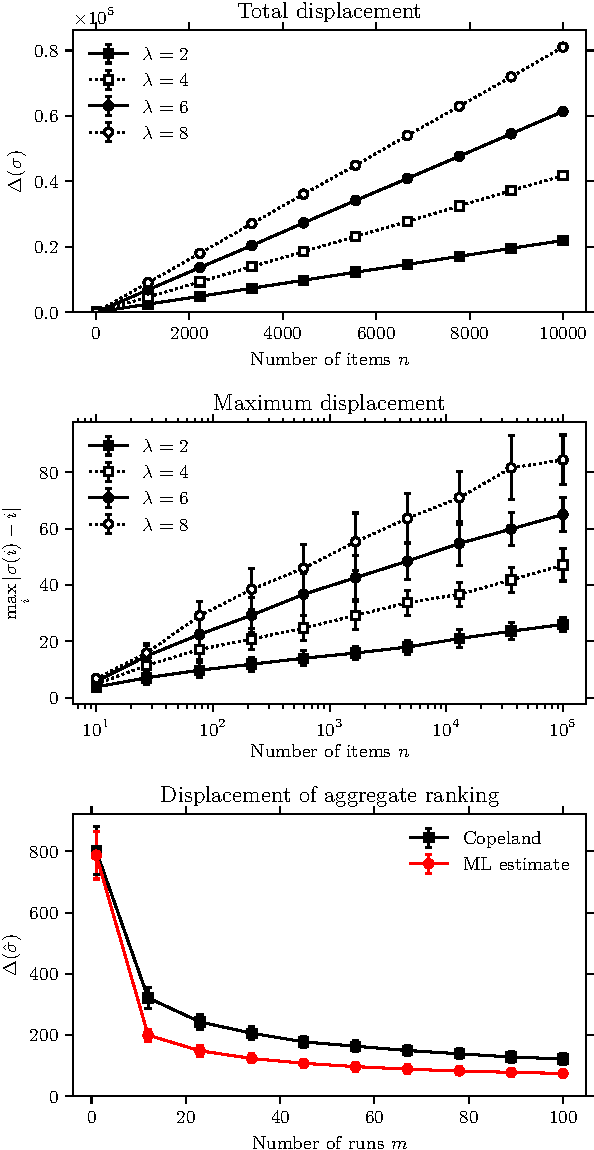
\includegraphics{rs-bounds}
\caption{
Empirical validation of Theorem~\ref{rs:thm:quickdisp} and illustration of Theorem~\ref{rs:thm:multidisp}.
Every simulation is repeated $50$ times, and we report the mean and the standard deviation.
Top and middle: total and maximum displacement (respectively) for increasing $N$ and different values of $\lambda$.
Bottom: displacement of the aggregate ranking $\hat{\sigma}$ for increasing $K$, fixing $N = \num{200}$ and $\lambda = \num{4}$ and using two different aggregation rules.
}
\label{rs:fig:bounds}
\end{figure}


%%%%%%%%%%%%%%%%%%%%%%%%%%%%%%%%%%%%%%%%%%%%%%%%%%%%%%%%%%%%%%%%%%%%%%%%%
\subsection{Independent Uniformly Distributed Parameters}
\label{rs:sec:iidunif}

A different (perhaps more natural) assumption about the parameters $\bm{\theta}$ is to consider that they are drawn independently and uniformly at random over some interval.
That is,
\begin{align*}
\text{i.i.d.}\; \bar{\theta}_1, \ldots, \bar{\theta}_N \sim \DUnif{0, (N+1) / \lambda},
\end{align*}
with $\theta_1, \ldots, \theta_N$ the order statistics of $\bar{\bm{\theta}}$, i.e., the random variables arranged in increasing order.
From some elementary results on the joint distribution of order statistics \citep[see, e.g.,][]{arnold2008first}, we have that
\begin{align*}
\Abs{\theta_{i+k} - \theta_{i}} \sim (N+1) / \lambda \cdot \DBeta{k, N - k + 1},
\end{align*}
i.e., $\Abs{\theta_{i+k} - \theta_{i}}$ is distributed as a Beta random variable rescaled between $0$ and $(N+1) / \lambda$.
Letting $f_{k,N}(x)$ be the probability density of $\Abs{\theta_{i+k} - \theta_{i}}$, we have, for any fixed $k$ and $\lambda$,
\begin{align*}
f_{k,N}(x) \propto x^{k-1} \left[ 1 - \frac{\lambda x}{N + 1} \right]^{N - k} \xrightarrow{N \to \infty} x^{k-1} e^{-\lambda x}.
\end{align*}
We recognize the functional form of the density of a \DGamma{k, \lambda} distribution.
Hence, the Poisson model and the i.i.d. uniform model are essentially equivalent for fixed $\lambda$ and large $N$, and we can expect the results developed in Section~\ref{rs:sec:poisson} to hold in the i.i.d. uniform case as well.

%%%%%%%%%%%%%%%%%%%%%%%%%%%%%%%%%%%%%%%%%%%%%%%%%%%%%%%%%%%%%%%%%%%%%%%%%
\section{Inference Algorithm}  %%%%%%%%%%%%%%%%%%%%%%%%%%%%%%%%%%%%%%%%%%
\label{cr:sec:algorithm}

The maximizer of the log-posterior does not have a closed-form solution.
In the spirit of the algorithms of \citet{hunter2004mm} for variants of Luce's choice model, we develop a minorization-maximization (MM) algorithm.
Simply put, the algorithm iteratively refines an estimate of the maximizer by solving a sequence of surrogates of the log-posterior.
Using the inequality $\log x \le \log \tilde{x} + x/\tilde{x} - 1$ (with equality if and only if $x = \tilde{x}$), we can lower-bound the log-posterior~\eqref{cr:eq:logpost} by
\begin{align*}
&f^{(t)}(\bm{\lambda}) =
    \sum_{i = 1}^n \bigg[ (c^-_i + \alpha - 1) \log \lambda_i 
                         - c^+_i \bigg( \log\!\sum_{k \in N^+_i}\!\lambda^{(t)}_k
                                       +\frac{\sum_{k \in N^+_i}\!\lambda_k}{\sum_{k \in N^+_i}\!\lambda^{(t)}_k} -1 \bigg)
                         - \beta \lambda_i \bigg] + \kappa,
\end{align*}
with equality if and only if $\bm{\lambda} = \bm{\lambda}^{(t)}$.
Starting with an arbitrary $\bm{\lambda}^{(0)} \in \mathbf{R}^n_{>0}$, we repeatedly solve the optimization problem
\begin{align*}
\bm{\lambda}^{(t+1)} = \Argmax_{\bm{\lambda}} f^{(t)}(\bm{\lambda}).
\end{align*}
Unlike the maximization of the log-posterior, the surrogate optimization problem has a closed-form solution, obtained by setting $\nabla f^{(t)}$ to $\bm{0}$:
\begin{align}
\label{cr:eq:mmiter}
\lambda_i^{(t + 1)} = \frac{c^-_i + \alpha - 1}{\sum_{j \in N^-_i} \gamma_j^{(t)} + \beta},
\ \gamma_j^{(t)} = \frac{c^+_j}{\sum_{k \in N^+_j} \lambda_k^{(t)}}.
\end{align}
The iterates provably converge to the maximizer of~\eqref{cr:eq:logpost}, as shown by the following theorem.

\begin{theorem}
\label{cr:thm:mmconv}
Let $\bm{\lambda}^\star$ be the unique maximum a-posteriori estimate.
Then for any initial $\bm{\lambda}^{(0)} \in \mathbf{R}^n_{> 0}$ the sequence of iterates defined by~\eqref{cr:eq:mmiter} converges to $\bm{\lambda}^\star$.
\end{theorem}

Theorem~\ref{cr:thm:mmconv} follows from a standard result on the convergence of MM algorithms and uses the fact that the log-posterior increases after each iteration.
Furthermore, it is known that MM algorithms exhibit geometric convergence in a neighborhood of the maximizer \citep{lange2000optimization}.
A thorough investigation of the convergence properties is left for future work.

\begin{algorithm}[t]
  \caption{ChoiceRank}
  \label{cr:alg:choicerank}
  \begin{algorithmic}[1]
    \Require graph $G = (V, E)$, counts $\{ (c^-_i, c^+_i) \}$
    \State $\bm{\lambda} \gets [1, \ldots, 1]$
    \Repeat
      \State $\bm{z} \gets \bm{0}_n$
      \Comment{Recompute $\bm{\gamma}$}
      \OneLineFor{$(i, j) \in E$} $z_i \gets z_i + \lambda_j$
      \OneLineFor{$i \in V$} $\gamma_i \gets c^+_i / z_i$
      \State $\bm{z} \gets \bm{0}_n$
      \Comment{Recompute $\bm{\lambda}$}
      \OneLineFor{$(i, j) \in E$} $z_j \gets z_j + \gamma_i$
      \OneLineFor{$i \in V$} $\lambda_i \gets (c^-_i + \alpha - 1) / (z_i + \beta)$
    \Until $\bm{\lambda}$ has converged
  \end{algorithmic}
\end{algorithm}
%In practice, we notice that adding a little bit of regularization through the Gamma prior greatly improves convergence.

The structure of the updates in~\eqref{cr:eq:mmiter} leads to an extremely simple and efficient implementation, given in Algorithm~\ref{cr:alg:choicerank}: we call it ChoiceRank.
A graphical representation of an iteration from the perspective of a single node is given in Figure~\ref{cr:fig:msgpassing}.
Each iteration consists of two phases of message passing, with $\gamma_i$ flowing towards in-neighbors $N^-_i$, then $\lambda_i$ flowing towards out-neighbors $N^+_i$.
The updates to a node's state are a function of the sum of the messages.
As the algorithm does two passes over the edges and two passes over the vertices, an iteration takes $\BigO{m + n}$ time.
The edges can be processed in any order, and the algorithm maintains a state over only $\BigO{n}$ values associated with the vertices.
Furthermore, the algorithm can be conveniently expressed in the well-known vertex-centric programming model \citep{malewicz2010pregel}.
This makes it easy to implement ChoiceRank inside scalable, optimized graph-processing systems such as Apache Spark \citep{gonzalez2014graphx}.

\begin{figure}[t]
  \centering
  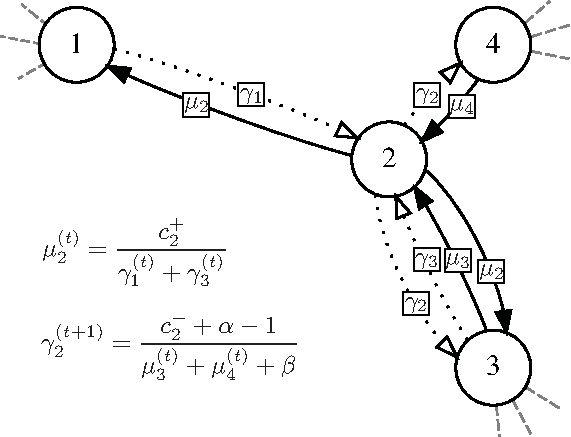
\includegraphics[width=0.5\linewidth]{cr-message-passing}
  \caption{One iteration of ChoiceRank from the perspective of node $2$.
  Messages flow in both directions along the edges of the graph $G$, first in the reverse direction (in dotted) then in the forward direction (in solid).}
  \label{cr:fig:msgpassing}
\end{figure}

\paragraph{EM Viewpoint}
The update~\eqref{cr:eq:mmiter} can also be explained from an expectation-maximization (EM) viewpoint, by introducing suitable latent variables \citep{caron2012efficient}.
This viewpoint enables a Gibbs sampler that can be used for Bayesian inference.
We present the EM derivation in Appendix~\ref{cr:app:algorithm}, but leave a study of fully Bayesian inference in the network choice model for future work.

%%%%%%%%%%%%%%%%%%%%%%%%%%%%%%%%%%%%%%%%%%%%%%%%%%%%%%%%%%%%%%%%%%%%%%%%%
\section{Experimental Evaluation}  %%%%%%%%%%%%%%%%%%%%%%%%%%%%%%%%%%%%%%
\label{cr:sec:experiments}

% Think of the difference between *predictive* and *explanatory*.
In this section, we investigate
\begin{enuminline}
\item the ability of the network choice model to accurately recover transitions in real-world scenarios, and
\item the potential of ChoiceRank to scale to very large networks.
\end{enuminline}

%%%%%%%%%%%%%%%%%%%%%%%%%%%%%%%%%%%%%%%%%%%%%%%%%%%%%%%%%%%%%%%%%%%%%%%%%
\subsection{Accuracy on Real-World Data}
\label{cr:sec:accuracy}

We evaluate the network choice model on three datasets that are representative of two distinct application domains.
%The first dataset contains clickstream data from the English Wikipedia, i.e., traces of users' navigation on a Web site.
%The second dataset consists of the records of all trips made using New York City's bicycle-sharing service during the year 2015, i.e., mobility traces in a large city.
Each dataset can be represented as a set of transition counts $\{ c_{ij} \}$ on a directed graph $\mathcal{G} = (\mathcal{V}, \mathcal{E})$.
We aggregate the transition counts into marginal traffic data $\{ (c^-_i, c^+_i) : i \in \mathcal{V} \}$ and fit a network choice model by using ChoiceRank (for simplicity, we set $w_{ij} \equiv 1$ for all datasets).
We set $\alpha = 2.0$ and $\beta = 1.0$ (these small values simply guarantee the convergence of the algorithm for any network structure) and declare convergence when $\Norm{\bm{\gamma}^{(t)} - \bm{\gamma}^{(t-1)}} / N < 10^{-8}$.
Given $\bm{\gamma}$, we estimate transition probabilities using $p_{ij} \propto \gamma_j$ as given by \eqref{cr:eq:singlelik}.
To the best of our knowledge, there is no other published method tackling the problem of estimating transition probabilities from marginal traffic data.
Therefore, we compare our method to three baselines based on simple heuristics.
\begin{description}
\item[Traffic] Transitions probabilities are proportional to the traffic of the target node: $q_{ij}^T \propto c_j^{-}$.
\item[PageRank] Transition probabilities are proportional to the PageRank score of the target node: $q_{ij}^P \propto \text{PR}_j$.
\item[Uniform] Any transition is equiprobable: $q_{ij}^U \propto 1$.
\end{description}
The four estimates are compared against ground-truth transition probabilities derived from the edge traffic data: $p_{ij}^\star \propto c_{ij}$.
We emphasize that although per-edge transition counts $\{c_{ij}\}$ are needed to \emph{evaluate} the accuracy of the network choice model (and the baselines), these counts are not necessary for \emph{learning} the model---per-node marginal counts are sufficient.

Given a node $i$, we measure the accuracy of a distribution $\bm{q}_i$ over outgoing transitions using two error metrics, the KL-divergence and the (normalized) rank displacement:
\begin{align*}
D_{\text{KL}}(\bm{p}_i^\star, \bm{q}_i) &= \sum_{j \in \mathcal{N}^+_i} p^\star_{ij} \log \frac{p^\star_{ij}}{q_{ij}}, \\
D_{\text{FR}}(\bm{p}_i^\star, \bm{q}_i) &= \frac{1}{\Abs{\mathcal{N}^+_i}^2} \sum_{j \in \mathcal{N}^+_i} \vert \sigma^\star_i(j) - \hat{\sigma}_i(j) \vert,
\end{align*}
where $\sigma^\star_i$ (respectively $\hat{\sigma}_i$) is the ranking of elements in $\mathcal{N}^+_i$ by decreasing order of $p^\star_{ij}$ (respectively $q_{ij}$).
We report the distribution of errors ``over choices'', i.e., the error at each node $i$ is weighted by the number of outgoing transitions $c^+_i$.


\subsubsection{Clickstream Data}

\paragraph{Wikipedia}
The Wikimedia Foundation has a long history of publicly sharing aggregate, page-level web traffic data\footnote{See: \url{https://stats.wikimedia.org/}.}.
Recently, it also released clickstream data from the English version of Wikipedia \citep{wulczyn2016wikipedia}, providing us with essential ground-truth transition-level data.
We consider a dataset that contains information, extracted from the server logs, about the traffic each page of the English Wikipedia received during the month of March 2016.
Each page's incoming traffic is grouped by HTTP referrer, i.e., by the page visited prior to the request.
We ignore the traffic generated by external Web sites such as search engines and keep only the internal traffic (\num{18}\% of the total traffic in the dataset).
In summary, we obtain counts of transitions on the hyperlink graph of English Wikipedia articles.
The graph contains $N = \num{2316032}$ nodes and $M = \num{13181698}$ edges, and we consider slightly over \num{1.2} billion transitions over the edges.
On this dataset, ChoiceRank converges after \num{795} iterations.

\paragraph{Kosarak}
We also consider a second clickstream dataset from a Hungarian online news portal\footnote{The data is publicly available at \url{http://fimi.ua.ac.be/data/}.}.
The data consists of $\num{7029013}$ transitions on a graph containing $N = 41001$ nodes and $M = \num{974560}$ edges.
ChoiceRank converges after \num{625} iterations.

The four topmost plots of Figure~\ref{cr:fig:perf-combined} show the error distributions.
ChoiceRank significantly improves on the baselines, both in terms of KL-divergence and rank displacement.
These results give compelling evidence that transitions do not occur proportionally with the target's page traffic: in terms of KL-divergence, ChoiceRank improves on Traffic by a factor $3\times$ and $2\times$, respectively.
PageRank scores, while reflecting some notion of importance of a page, are not designed to estimate transitions, and understandably the corresponding baseline performs poorly.
Uniform (perhaps the simplest of our baselines) is (by design) unable to distinguish among transitions, resulting in a large displacement error.
We believe that its comparatively better performance in terms of KL-divergence (for Wikipedia) is mostly an artifact of the metric, which encourages ``prudent'' estimates.
Finally, in Figure~\ref{cr:fig:perf-wikipedia} we observe that ChoiceRank seems to perform comparatively better as the number of possible transition increases.

\begin{figure}
  \centering
  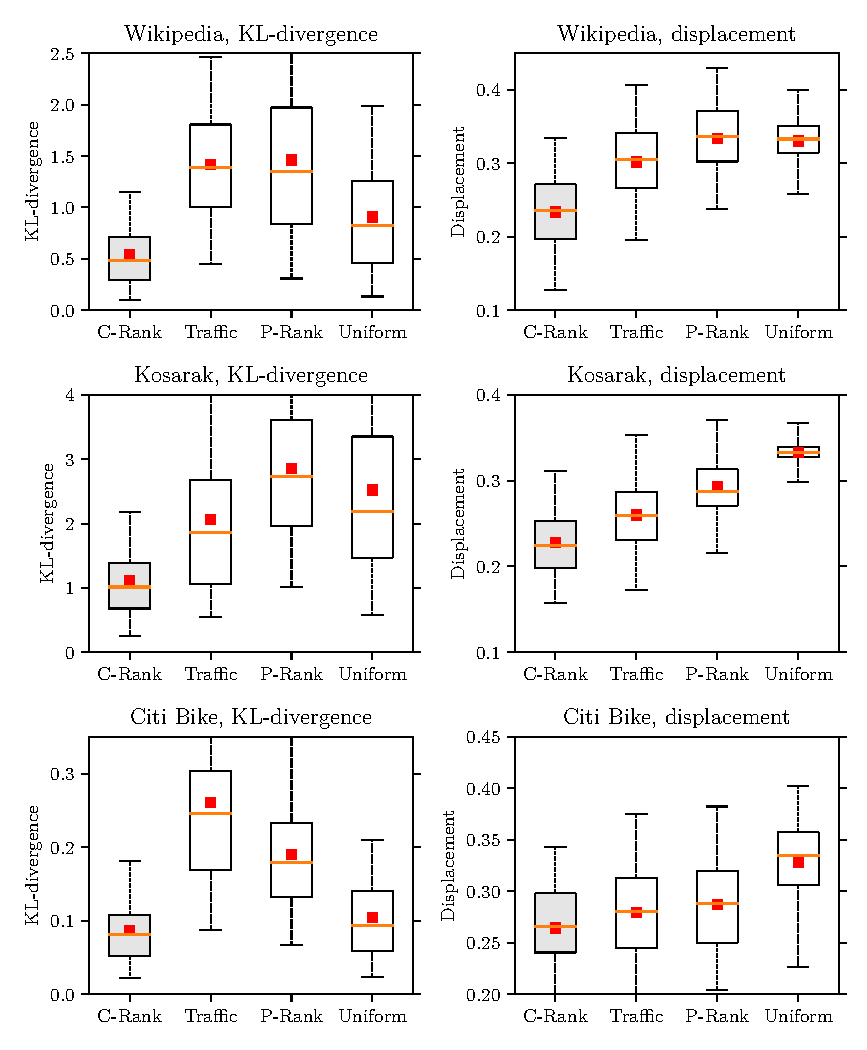
\includegraphics{cr-perf-combined}
  \caption{
Error distributions of the network choice model and three baselines for the Wikipedia, Kosarak and Citi Bike datasets.
The boxes show the interquartile range, the whiskers show the $5^{\text{th}}$ and $95^{\text{th}}$ percentiles, the red horizontal bars show the median and the red squares show the mean.
}
  \label{cr:fig:perf-combined}
\end{figure}

\begin{figure}
  \centering
  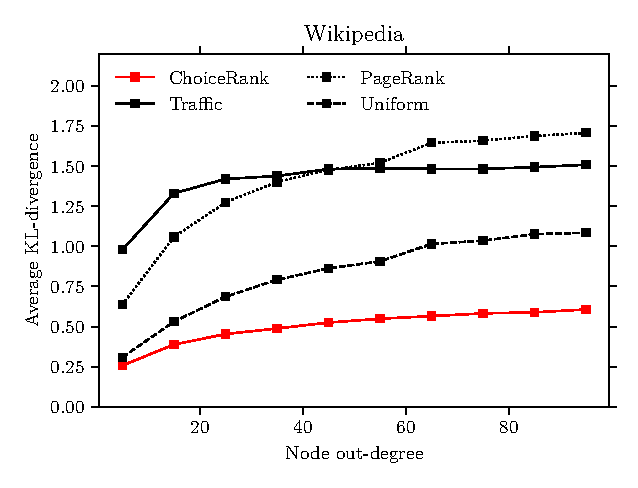
\includegraphics{cr-perf-wikipedia}
  \caption{
Average KL-divergence as a function of the number of possible transitions for the Wikipedia dataset.
ChoiceRank performs comparatively better in the case where a node's out-degree is large.
}
  \label{cr:fig:perf-wikipedia}
\end{figure}


\subsubsection{NYC Bicycle-Sharing Data}

Next, we consider trip data from Citi Bike, New York City's bicycle-sharing system\footnote{The data is available at \url{https://www.citibikenyc.com/system-data}.}.
%Markov models have been used with success in the context of mobility prediction \citep{ashbrook2003using, kafsi2015traveling}. TODO
For each ride on the system made during the year 2015, we extract the pick-up and drop-off stations and the duration of the ride.
Because we want to focus on direct trips, we exclude rides that last more than one hour.
We also exclude source-destinations pairs which have less than 1 ride per day on average (a majority of source-destination pairs appears at least once in the dataset).
The resulting data consists of \num{3.4} million rides on a graph containing $N = \num{497}$ nodes and $M = \num{5209}$ edges.
ChoiceRank converges after $\num{7508}$ iterations.
We compute the error distribution in the same way as for the clickstream datasets.

The two bottommost plots of Figure~\ref{cr:fig:perf-combined} display the results.
The observations made on the clickstream datasets carry over to this mobility dataset, albeit to a lesser degree.
A significant difference between clicking a link and taking a bicycle trip is that in the latter case, there is a non-uniform ``cost'' of a transition due to the distance between source and target.
In future work, one might consider experimenting with edge weights $\{ w_{ij} \}$ that capture this.


%%%%%%%%%%%%%%%%%%%%%%%%%%%%%%%%%%%%%%%%%%%%%%%%%%%%%%%%%%%%%%%%%%%%%%%%%
\subsection{Scaling to Large Networks}

To demonstrate ChoiceRank's scalability, we develop a simple implementation in the Rust programming language, based on the ideas of COST \citep{mcsherry2015scalability}.
Our code is publicly available online\footnote{See: \url{https://github.com/lucasmaystre/choicerank}.}.
The implementation repeatedly streams edges from disk and keeps four floating-point values per node in memory:
the counts $c^-_i$ and $c^+_i$, the sum of messages $z_i$, and either $\mu_i$ or $\gamma_i$ (depending on the stage in the iteration).
As edges can be processed in any order, it can be beneficial to reorder the edges in a way that accelerates the computation.
For this reason, our implementation preprocesses the list of edges and reorders them in Hilbert curve order\footnote{A Hilbert space-filling curve visits all the entries of the adjacency matrix of the graph, in a way that preserves locality of both source and destination of the edges.}.
This results in better cache locality and yields a significant speedup.

We test our implementation on a hyperlink graph extracted from the 2012 Common Crawl web corpus\footnote{
The data is available at \url{http://webdatacommons.org/hyperlinkgraph/}.} that contains over \num{3.5} billion nodes and \num{128} billion edges \citep{meusel2014graph}.
The edge list alone requires about $1$ TB of uncompressed storage.
There is no publicly available information on the traffic at each page, therefore we generate a value $c_i$ for every node $i$ randomly and uniformly between \num{100} and \num{500}, and set both $c^-_i$ and $c^+_i$ to $c_i$.
As such, this experiment does not attempt to measure the validity of the model (unlike the experiments of Section~\ref{cr:sec:accuracy}).
Instead, it focuses on testing the algorithm's potential to scale to very large networks.

\paragraph{Results}
We run \num{20} iterations of ChoiceRank on a dual Intel Xeon E5-2680 v3 machine, with \num{256} GB of RAM and \num{6} HDDs configured in RAID 0.
We arbitrarily set $\alpha = 2.0$ and $\beta = 1.0$ (but this choice has no impact on the results).
Only about \num{65} GB of memory is used, all to store the nodes' state ($4 \times 4$ bytes per node).
The algorithm takes a little less than \num{39} minutes per iteration on average.
Collectively, these results validate the feasibility of model inference for very large datasets.

It is worth noting that despite tackling different problems, the ChoiceRank algorithm exhibits interesting similarities with a message-passing implementation of PageRank commonly used in scalable graph-parallel systems such as Pregel \citep{malewicz2010pregel} and Spark \citep{gonzalez2014graphx}.
For comparison, using the COST code \citep{mcsherry2015scalability} we run \num{20} iterations of PageRank on the same hardware and data.
PageRank uses slightly less memory (about \num{50} GB, or one less floating-point number per node) and takes about half of the time per iteration (a little over \num{20} minutes).
This is consistent with the fact that ChoiceRank requires two passes over the edges per iteration, whereas PageRank requires one.
The similarities between the two algorithms lead us to believe that ChoiceRank can benefit from any new system optimization developed for PageRank.

%%%%%%%%%%%%%%%%%%%%%%%%%%%%%%%%%%%%%%%%%%%%%%%%%%%%%%%%%%%%%%%%%%%%%%%%%
\section{Summary}  %%%%%%%%%%%%%%%%%%%%%%%%%%%%%%%%%%%%%%%%%%%%%%%%%%%%%%
\label{cr:sec:summary}

In this chapter, we present a method that tackles the problem of finding the transition probabilities along the edges of a network, given only the network's structure and aggregate node-level traffic data.
This method generalizes and extends ideas recently presented by \citet{kumar2015inverting}.
We demonstrate that in spite of the strong model assumptions needed to learn $\BigO{n^2}$ probabilities from $\BigO{n}$ observations, the method still manages to recover the transition probabilities to a good level of accuracy on two clickstream datasets, and shows promise for applications beyond clickstream data.
To sum up, we believe that our method will be useful to pracitioners interested in understanding patterns of navigation in networks from aggregate traffic data, commonly available, e.g., in public datasets.


%%%%%%%%%%%%%%%%%%%%%%%%%%%%%%%%%%%%%%%%%%%%%%%%%%%%%%%%%%%%%%%%%%%%%%%%%
\section{Extensions and Proofs}  %%%%%%%%%%%%%%%%%%%%%%%%%%%%%%%%%%%%%%%%
\label{cr:app:extensions}

In this section, we start by generalizing the network choice model to account for edge weights.
Then, we present formal proofs for
\begin{enuminline}
\item the (minimal) sufficiency of marginal counts and
\item the well-posedness of MAP inference
\end{enuminline}
in the generalized weighted network choice model.

%%%%%%%%%%%%%%%%%%%%%%%%%%%%%%%%%%%%%%%%%%%%%%%%%%%%%%%%%%%%%%%%%%%%%%%%%
\subsection{Generalization of the Model}

Let $\mathcal{G} = (\mathcal{V}, \mathcal{E})$ be a weighted, directed graph with edge weights $w_{ij} > 0$ for all $(i, j) \in \mathcal{E}$.
\citet{kumar2015inverting} propose the following generalization of Luce's choice model.
Given a parameter vector $\bm{\gamma} \in \mathbf{R}_{>0}^N$, they define the choice probabilities as
\begin{align}
\label{cr:eq:wsinglelik}
p_{ij} = \frac{w_{ij} \gamma_j}{\sum_{k \in \mathcal{N}^+_i} w_{ik} \gamma_k}, \quad j \in \mathcal{N}^+_i.
\end{align}
We refer to this model as the \emph{weighted network choice model}.
Intuitively, the strength of each alternative is weighted by the corresponding edge's weight;
Luce's original choice model is obtained by setting $w_{ij} = \text{constant}$.
In this general model, the log-likelihood becomes
\begin{align}
\ell(\bm{\gamma} ; \mathcal{D})
    &= \sum_{(i,j) \in \mathcal{E}} c_{ij} \bigg[ \log w_{ij} \gamma_j - \log \sum_{k \in \mathcal{N}^+_i} w_{ik} \gamma_k \bigg] \nonumber \\
    &= \sum_{(i,j) \in \mathcal{E}} c_{ij} \bigg[ \log \gamma_j - \log \sum_{k \in \mathcal{N}^+_i} w_{ik} \gamma_k \bigg] \nonumber
       + \sum_{(i,j) \in \mathcal{E}} c_{ij} \log w_{ij}, \nonumber \\
    &= \sum_{i = 1}^N \bigg[ c^-_i \log \gamma_i - c^+_i \log\!\sum_{k \in \mathcal{N}^+_i}\!w_{ik} \gamma_k \bigg] + \kappa_1, \label{cr:eq:wloglik}
\end{align}
where $c^-_i = \sum_{j \in \mathcal{N}^-_i} c_{ji}$ and $c^+_i = \sum_{j \in \mathcal{N}^+_i} c_{ij}$ is the aggregate number of transitions arriving in and originating from $i$, respectively.
Note that for every $i$, the weights $\{ w_{ij} : j \in \mathcal{N}^+_i \}$ are equivalent up to rescaling.

This generalization is relevant in situations where the current context modulates the alternatives' strength.
For example, this could be used to take into account the position or prominence of a link on a page in a hyperlink graph, or the distance between two locations in a mobility network.


%%%%%%%%%%%%%%%%%%%%%%%%%%%%%%%%%%%%%%%%%%%%%%%%%%%%%%%%%%%%%%%%%%%%%%%%%
\subsection{Minimal Sufficiency of Marginal Counts}

Recall that $c_{ij}$ denotes the number of times we observe a transition from $i$ to $j$.
We set out to prove the following theorem for the weighted network choice model.

\begin{theorem}
Let $c^-_i = \sum_{j \in \mathcal{N}^-_i} c_{ji}$ and $c^+_i = \sum_{j \in \mathcal{N}^+_i} c_{ij}$ be the aggregate number of transitions arriving in and originating from $i$, respectively.
Then, $\{ (c^-_i, c^+_i) : i \in \mathcal{V} \}$ is a minimally sufficient statistic for the parameters $\bm{\gamma}$ in the weighted network choice model.
\end{theorem}

\begin{proof}
Let $f(\{ c_{ij} \} \mid \bm{\gamma})$ be the discrete probability density function of the data under the model with parameters $\bm{\gamma}$.
Theorem $6.2.13$ in \citet{casella2002statistical} states that $\{ (c^-_i, c^+_i) \}$ is a minimally sufficient statistic for $\bm{\gamma}$ if and only if, for any $\{ c_{ij} \}$ and $\{ d_{ij} \}$ in the support of $f$,
\begin{align}
\label{cr:eq:minsuff}
\begin{aligned}
\frac{ f(\{ c_{ij} \} \mid \bm{\gamma}) }{ f(\{ d_{ij} \} \mid \bm{\gamma}) }\ \text{is independent of $\bm{\gamma}$}
\iff (c^-_i, c^+_i) = (d^-_i, d^+_i) \quad \forall i.
\end{aligned}
\end{align}
Taking the log of the ratio on the left-hand side and using~\eqref{cr:eq:wloglik}, we find that
\begin{align*}
\log \frac{ f(\{ c_{ij} \} \mid \bm{\gamma}) }{ f(\{ d_{ij} \} \mid \bm{\gamma}) } =
  \sum_{i = 1}^N \bigg[ (c^-_i\!-\!d^-_i) \log \gamma_i
                       - (c^+_i\!-\!d^+_i) \log\!\sum_{k \in \mathcal{N}^+_i}\!w_{ik} \gamma_k \bigg] + \kappa_2.
\end{align*}
From this, it is easy to see that the ratio of densities is independent of $\bm{\gamma}$ if and only if $c^-_i = d^-_i$ and $c^+_i = d^+_i$, which verifies~\eqref{cr:eq:minsuff}.
\end{proof}

%%%%%%%%%%%%%%%%%%%%%%%%%%%%%%%%%%%%%%%%%%%%%%%%%%%%%%%%%%%%%%%%%%%%%%%%%
\subsection{Well-Posedness of MAP Inference}

Using a $\text{Gamma}(\alpha, \beta)$ prior for each parameter, the log-posterior of the weighted network choice model can be written as
\begin{align}
\label{cr:eq:wlogpost}
\begin{aligned}
&\log p(\bm{\gamma} \mid \mathcal{D}) =
    \sum_{i = 1}^N \bigg[ (c^-_i + \alpha - 1) \log \gamma_i
        - c^+_i \log \bigg( \sum_{k \in \mathcal{N}^+_i} w_{ik} \gamma_k \bigg)  - \beta \gamma_i \bigg]
    + \kappa_3.
\end{aligned}
\end{align}
We prove a theorem that guarantees that MAP estimation is well-posed in this generalized model; the proof of Theorem~\ref{cr:thm:map} follows trivially.

\begin{theorem}
\label{cr:thm:wmap}
If i.i.d. $\gamma_1, \ldots, \gamma_N \sim \text{Gamma}(\alpha, \beta)$ with $\alpha > 1$, then there exists a unique maximizer $\bm{\gamma}^\star \in \mathbf{R}^N_{>0}$ of the weighted network choice model's log-posterior~\eqref{cr:eq:wlogpost}.
\end{theorem}

\begin{proof}
The log-posterior~\eqref{cr:eq:wlogpost} is not concave in $\bm{\gamma}$, but it can be made concave using the simple reparametrization $\gamma_i = e^{\theta_i}$.
Under this reparametrization, the log-prior and the log-likelihood become
\begin{align*}
\log p(\bm{\theta})
    &= \sum_{i = 1}^N \left[ (\alpha - 1) \theta_i - \beta e^{\theta_i} \right] + \kappa_4, \\
\ell(\bm{\theta} ; \mathcal{D})
    &= \sum_{i = 1}^N \bigg[ c^-_i \theta_i - c^+_i \log \sum_{k \in \mathcal{N}^+_i} w_{ik} e^{\theta_k} \bigg] + \kappa_5.
\end{align*}
It is easy to see that the log-likelihood is concave and the log-prior strictly concave in $\bm{\theta}$.
As a result, the log-posterior is strictly concave in $\bm{\theta}$, which ensures that there exists at most one maximizer.

Now consider any transition counts $\{ c_{ij} \}$ that satisfy $c^-_i = \sum_{j \in \mathcal{N}^-_i} c_{ji}$ and $c^+_i = \sum_{j \in \mathcal{N}^+_i} c_{ij}$.
The log-posterior can be written as
\begin{align*}
\log p(\bm{\theta} \mid \mathcal{D})
    &= \sum_{i = 1}^N \sum_{j \in \mathcal{N}^+_i} c_{ij} \bigg[ \theta_j - \log \sum_{k \in \mathcal{N}^+_i} w_{ik} e^{\theta_k} \bigg]
       + \sum_{i = 1}^N \left[ (\alpha - 1) \theta_i - \beta e^{\theta_i} \right] + \kappa_3\\
    &\le -N^2 \cdot \max_{i,j} \log w_{ij}
       + \sum_{i = 1}^N \left[ (\alpha - 1) \theta_i - \beta e^{\theta_i} \right] + \kappa_3.
\end{align*}
For $\alpha > 1$, it follows that $\lim_{\Norm{\bm{\theta}} \to \infty} \log p(\bm{\theta} \mid \mathcal{D}) = -\infty$, which ensures that there is at least one maximizer.
\end{proof}

Note that Theorem~\ref{cr:thm:wmap} can easily be extended to independent but non-identical Gamma priors, where $\gamma_i \sim \text{Gamma}(\alpha_i, \beta_i)$ and $\alpha_i \ne \alpha_j$, $\beta_i \ne \beta_j$ in general.

%%%%%%%%%%%%%%%%%%%%%%%%%%%%%%%%%%%%%%%%%%%%%%%%%%%%%%%%%%%%%%%%%%%%%%%%%
\section{Maximum-Likelihood Estimation}  %%%%%%%%%%%%%%%%%%%%%%%%%%%%%%%%
\label{cr:app:maxlik}

In this section, we go into the analysis of the ML estimator in depth.
From the definition of choice probabilities in~\eqref{cr:eq:wsinglelik}, it is clear that the likelihood is invariant to a rescaling of the parameters, i.e., $\ell(\bm{\lambda}; \mathcal{D}) = \ell(s \bm{\lambda}; \mathcal{D})$ for any $s > 0$.
We will therefore identify parameters up to rescaling.

%%%%%%%%%%%%%%%%%%%%%%%%%%%%%%%%%%%%%%%%%%%%%%%%%%%%%%%%%%%%%%%%%%%%%%%%%
\subsection{Necessary and Sufficient Conditions}

In order to provide a data-dependent, necessary and sufficient condition that guarantees that the ML estimate is well-defined, we extend the definition of comparison hypergraph presented in Section~\ref{cr:sec:maxlik}.

\begin{definition}[comparison graph]
Let $G = (V, E)$ be a directed graph and $\{ a_{ij} \mid (i,j) \in E \}$ be non-negative numbers.
The \emph{comparison graph} induced by $\{ a_{ij} \}$ is the directed graph $H = (V, E')$, where $(i,j) \in E'$ if and only if there is a node $k$ such that $i, j \in N^+_k$ and $a_{kj} > 0$.
\end{definition}

The numbers $\{ a_{ij}\}$ can be loosely interpreted as transition counts (although they do not need to be integer).
Intuitively, there is an edge $(i, j)$ in the comparison graph whenever there is at least one instance in which $i$ and $j$ were among the alternatives and $j$ was selected.
If $a_{ij} > 0$ for all edges, then the comparison graph is equivalent to its hypergraph counterpart, in that every hyperedge induces a clique in the comparison graph.
As shown by the next theorem, the notion of (data-dependent) comparison graph leads to a precise characterization of whether the ML estimate is well-defined or not.

\begin{theorem}
\label{cr:thm:mlboth}
Let $G = (V, E)$ be a directed graph and $\{ (c^-_i, c^+_i) \}$ be the aggregate number of transitions arriving in and originating from $i$, respectively.
Let $\{ a_{ij} \}$ be any set of non-negative real numbers that satisfy
\begin{align*}
\sum_{j \in N^-_i} a_{ji} = c^-_i, \quad
\sum_{j \in N^+_i} a_{ij} = c^+_i.
\end{align*}
Then, the maximizer of the log-likelihood~\eqref{cr:eq:wloglik} exists and is unique (up to rescaling) if and only if the comparison graph induced by $\{ a_{ij} \}$ is strongly connected.
\end{theorem}

The proof borrows from \citet{hunter2004mm}, in particular from the proofs of Lemmas~$1$ and~$2$.

\begin{proof}
The log-likelihood~\eqref{cr:eq:wloglik} is not concave in $\bm{\lambda}$, but it can be made concave using the reparametrization $\lambda_i = e^{\theta_i}$.
We can rewrite the reparametrized log-likelihood using $\{ a_{ij} \}$ as
\begin{align*}
    \ell(\bm{\theta})
        = \sum_{i = 1}^n \sum_{j \in N^+_i} a_{ij} \bigg[ \theta_j - \log \sum_{k \in N^+_i} w_{ik} e^{\theta_k} \bigg],
\end{align*}
and, without loss of generality, we can assume that $\sum_i \theta_i = 0$ and $\min_{ij} w_{ij} = 1$.

First, we shall prove that the super-level set $\{ \bm{\theta} \mid \ell(\bm{\theta}) \ge c \}$ is bounded and compact for any $c$, if and only if the comparison graph is strongly connected.
The compactness of all super-level sets ensures that there is at least one maximizer.
Pick any unit vector $\bm{u}$ such that $\sum_i u_i = 0$, and let $\bm{\theta} = s \bm{u}$
When $s \to \infty$, then $e^{\theta_i} > 0$ and $e^{\theta_j} \to 0 $ for some $i$ and $j$.
As the comparison graph is strongly connected, there is a path from $i$ to $j$, and along this path there must be two consecutive nodes $i', j'$ such that $e^{\theta_{i'}} > 0$ and $e^{\theta_{j'}} \to 0$.
The existence of the edge $(i',j')$ in the comparison graph means that there is a $k$ such that $i', j' \in N^+_k$ and $a_{kj'} > 0$.
Therefore, the log-likelihood can be bounded as
\begin{align*}
\ell(\bm{\theta})
    \le a_{kj'} \bigg[ \theta_{j'} - \log \sum_{q \in N^+_k} w_{kq} e^{\theta_q} \bigg]
    \le a_{kj'} \left[ \theta_{j'} - \log (e^{\theta_{j'}} + e^{\theta_{i'}}) \right],
\end{align*}
and $\lim_{s \to \infty} \ell(\bm{\theta}) = -\infty$.
Conversely, suppose that the comparison graph is not strongly connected and partition the vertices into two non-empty subsets $S$ and $T$ such that there is no edge from $S$ to $T$.
Let $c > 0$ be any positive constant, and take $\tilde{\theta}_i = \theta_i + c$ if $i \in S$ and $\tilde{\theta}_i = \theta_i$ if $i \in T$ (renormalize such that $\sum_i \tilde{\theta}_i = 0$).
Clearly, $\ell(\tilde{\bm{\theta}}) \ge \ell(\bm{\theta})$, and by repeating this procedure $\lVert \bm{\theta} \rVert$ may be driven to infinity without decreasing the likelihood.

Second, we shall prove that if the comparison graph is strongly connected, the log-likelihood is strictly concave (in $\bm{\theta}$).
In particular, for any $p \in (0,1)$,
\begin{align}
\label{cr:eq:strictconcav}
\ell \left[ p \bm{\theta} + (1-p) \bm{\eta} \right] \ge p \ell(\bm{\theta}) + (1-p) \ell(\bm{\eta}),
\end{align}
with equality if and only if $\bm{\theta} \equiv \bm{\eta}$ up to a constant shift.
Strict concavity ensures that there is at most one maximizer of log-likelihood.
We start with Hölder's inequality, which implies that, for positive $\{ x_k \}$ and $\{ y_k \}$, and $p \in (0,1)$,
\begin{align*}
\log \sum_k x_k^p y_k^{1-p} \le p \log \sum_k x_k + (1-p) \log \sum_k y_k.
\end{align*}
with equality if and only $x_k = c y_k$ for some $c > 0$.
Letting $x_k = w_{ik} e^{\theta_k}$ and $y_k = w_{ik} e^{\eta_k}$, we find that for all $i$
\begin{align}
\label{cr:eq:holderapp}
\begin{aligned}
\log \sum_{k \in N^+_i} w_{ik} e^{p \theta_k + (1-p) \eta_k}
    \le p \log\!\sum_{k \in N^+_i}\!w_{ik} e^{\theta_k} + (1-p) \log\!\sum_{k \in N^+_i}\!w_{ik} e^{\eta_k},
\end{aligned}
\end{align}
with equality if and only if there exists $c \in \mathbf{R}$ such that $\theta_k = \eta_k + c$ for all $k \in N^+_{i}$.
Multiplying by $a_{ij}$ and summing over $i$ and $j$ on both sides of~\eqref{cr:eq:holderapp} shows that the log-likelihood is concave in $\bm{\theta}$.
Now, consider any partition of the vertices into two non-empty subsets $S$ and $T$.
Because the comparison graph is strongly connected, there is always $k \in V$, $i \in S$ and $j \in T$ such that $i, j \in N^+_k$ and $a_{ki} > 0$.
Therefore, the left and right side of~\eqref{cr:eq:strictconcav} are equal if and only if $\bm{\theta} \equiv \bm{\eta}$ up to a constant shift.

Bounded super-level sets and strict concavity form necessary and sufficient conditions for the existence and uniqueness of the maximizer.
\end{proof}

We now give a proof for Theorem~\ref{cr:thm:mlnecessary}, presented in the main body of text.

\begin{proof}[Proof of Theorem~\ref{cr:thm:mlnecessary}]
If the comparison hypergraph is disconnected, then for any data $\mathcal{D}$, the (data-induced) comparison graph is disconnected too.
Furthermore, the connected components of the comparison graph are subsets of those of the hypergraph.
Partition the vertices into two non-empty subsets $S$ and $T$ such that there is no hyperedge between $S$ to $T$ in the comparison hypergraph.
Let $A = \{ i \mid N^+_i \subset S \}$ and $B = \{ i \mid N^+_i \subset T \}$.
By construction of the comparison hypergraph, $A \cap B = \varnothing$ and $A \cup B = V$.
The log-likelihood can be therefore be rewritten as
\begin{align*}
\ell(\bm{\theta}) =
    \sum_{i \in A} \sum_{j \in N^+_i} a_{ij} \bigg[ \log \lambda_j - \log \sum_{k \in N^+_i} w_{ik} \lambda_k \bigg]
    + \sum_{i \in B} \sum_{j \in N^+_i} a_{ij} \bigg[ \log \lambda_j - \log \sum_{k \in N^+_i} w_{ik} \lambda_k \bigg].
\end{align*}
The sum over $A$ involves only parameters related to nodes in $S$, while the sum over $B$ involves only parameters related to nodes in $T$.
Because the likelihood is invariant to a rescaling of the parameters, it is easy to see that we can arbitrarily rescale the parameters of the vertices in either $S$ or $T$ without affecting the likelihood.
\end{proof}

\begin{figure*}[t]
  \begin{subfigure}{.33\textwidth}
    \centering
    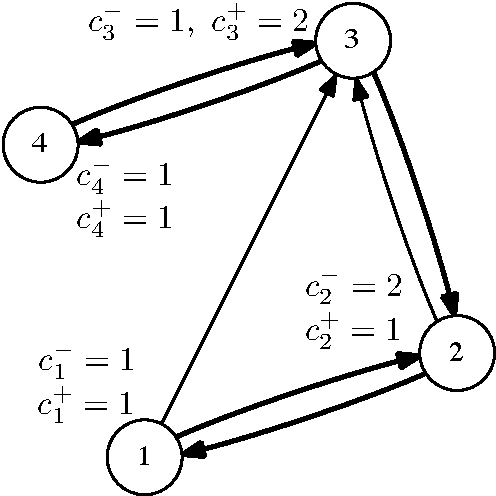
\includegraphics[width=.85\linewidth]{cr-ml-undefined}
    \caption{network structure}
  \end{subfigure}%
  \begin{subfigure}{.33\textwidth}
    \centering
    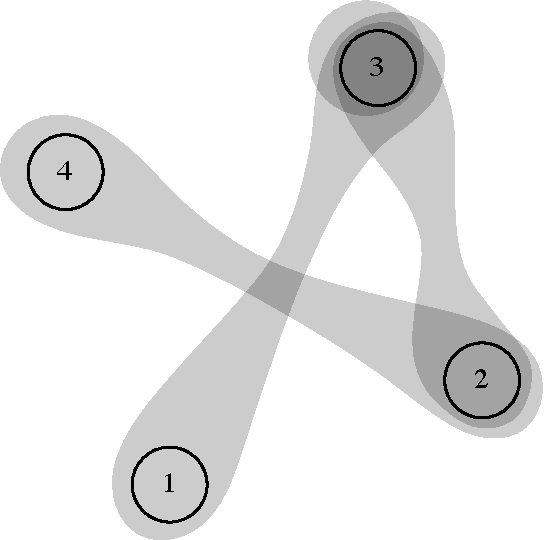
\includegraphics[width=.85\linewidth]{cr-ml-undefined-hyp}
    \caption{comparison hypergraph}
  \end{subfigure}
  \begin{subfigure}{.33\textwidth}
    \centering
    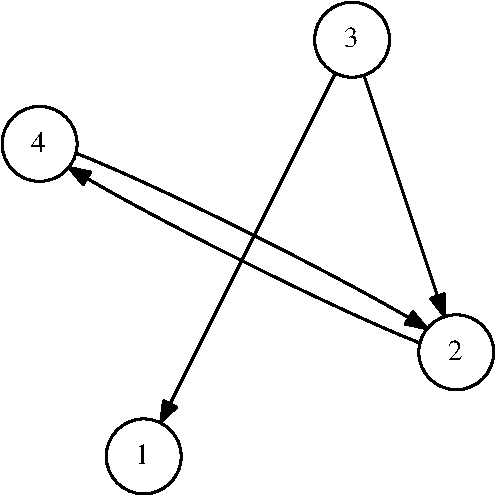
\includegraphics[width=.85\linewidth]{cr-ml-undefined-comp}
    \caption{comparison graph}
  \end{subfigure}
  \caption{An innocent-looking example where the ML estimate does not exist.
  The network structure, aggregate traffic data and compatible transitions are shown on the left.
  While the comparison hypergraph is connected, the (data-dependent) comparison graph is not strongly connected.}
  \label{cr:fig:badexample}
\end{figure*}

\paragraph{Verifying the Condition of Theorem~\ref{cr:thm:mlboth}}
In order to verify the necessary and sufficient condition given $\{ (c^-_i, c^+_i) \}$, one has to find a non-negative solution $\{ a_{ij} \}$ to the system of equations
\begin{align*}
\sum_{j \in N^-_i} a_{ji} &= c^-_i, \\
\sum_{j \in N^+_i} a_{ij} &= c^+_i.
\end{align*}
\citet{dines1926positive} presents a remarkably simple algorithm to find such a non-negative solution.
Alternatively, \citet{kumar2015inverting} suggest recasting the problem as one of maximum flow in a network.
However, the computational cost of running \citeauthor{dines1926positive}' or max-flow algorithms is significantly greater than that of running ChoiceRank.

\subsection{Example}

To conclude our discussion, we provide an innocuous-looking example that highlights the difficulty of dealing with the ML estimate.
Consider the network structure and traffic data depicted in Figure~\ref{cr:fig:badexample}.
The network is strongly connected, and its comparison hypergraph is connected as well; as such, the network satisfies the necessary condition stated in Theorem~\ref{cr:thm:mlnecessary} in the main text.
Nevertheless, the condition is not sufficient for the ML-estimate to be well-defined.
In this example, the (data-dependent) comparison graph is \emph{not} strongly connected, and it is easy to see that the likelihood can always be increased by increasing $\lambda_1$, $\lambda_2$ and $\lambda_4$.
Hence, the ML estimate does not exist.

In this simple example, we indicate the edge transitions that generated the observed marginal traffic in bold.
Given this information, the comparison graph is easy to find, and the necessary and sufficient conditions of Theorem~\ref{cr:thm:mlboth} are easy to check.
But in general, finding a set of transitions that is compatible with given marginal per-node traffic data is computationally expensive (see discussion above).

%%%%%%%%%%%%%%%%%%%%%%%%%%%%%%%%%%%%%%%%%%%%%%%%%%%%%%%%%%%%%%%%%%%%%%%%%
\section{ChoiceRank Algorithm}  %%%%%%%%%%%%%%%%%%%%%%%%%%%%%%%%%%%%%%%%%
\label{cr:app:algorithm}

In this section, we start by generalizing the ChoiceRank algorithm to the weighted network choice model.
We then prove the convergence of this generalized algorithm.
Finally, we show how the same algorithm can be obtained from an EM viewpoint by introducing suitable latent variables.

%%%%%%%%%%%%%%%%%%%%%%%%%%%%%%%%%%%%%%%%%%%%%%%%%%%%%%%%%%%%%%%%%%%%%%%%%
\subsection{Algorithm for the Generalized Model}

Using the same linear upper-bound on the logarithm as in Section~\ref{cr:sec:algorithm} of the main text, we can lower-bound the log-posterior~\eqref{cr:eq:wlogpost} in the weighted model by
\begin{align}
\label{cr:eq:wminorizing}
\begin{aligned}
f^{(t)}(\bm{\gamma}) = \kappa_2 + \sum_{i = 1}^N \bigg[
    & (c^-_i + \alpha - 1) \log \gamma_i - \beta \gamma_i \\
    &- c^+_i \bigg( \log\!\sum_{k \in \mathcal{N}^+_i}\!w_{ik} \gamma^{(t)}_k
                   +\frac{\sum_{k \in \mathcal{N}^+_i}\!w_{ik} \gamma_k}{\sum_{k \in \mathcal{N}^+_i}\!w_{ik} \gamma^{(t)}_k} -1 \bigg) \bigg],
\end{aligned}
\end{align}
with equality if and only if $\bm{\gamma} = \bm{\gamma}^{(t)}$.
Starting with an arbitrary $\bm{\gamma}^{(0)} \in \mathbf{R}^N_{>0}$, we repeatedly maximize the lower-bound $f^{(t)}$.
This surrogate optimization problem has a closed form solution, obtained by setting $\nabla f^{(t)}$ to $0$:
\begin{align}
\label{cr:eq:wmmiter}
\gamma_i^{(t + 1)} = \frac{c^-_i + \alpha - 1}{\sum_{j \in \mathcal{N}^-_i} w_{ji} \mu_j^{(t)} + \beta},
    \quad \text{where }
    \mu_j^{(t)} = \frac{c^+_j}{\sum_{k \in \mathcal{N}^+_j} w_{jk} \gamma_k^{(t)}}.
\end{align}
The iterates provably converge to the maximizer of~\eqref{cr:eq:wlogpost}, as shown by the following theorem.

\begin{theorem}
\label{cr:thm:wmmconv}
Let $\bm{\gamma}^\star$ be the unique maximum a-posteriori estimate.
Then for any initial $\bm{\gamma}^{(0)} \in \mathbf{R}^N_{> 0}$ the sequence of iterates defined by~\eqref{cr:eq:wmmiter} converges to $\bm{\gamma}^\star$.
\end{theorem}

The proof follows that of \citeauthor{hunter2004mm}'s Theorem~$1$ \citeyearpar{hunter2004mm}.

\begin{proof}
Let $M: \mathbf{R}^N_{>0} \to \mathbf{R}^N_{>0}$ be the (continuous) map implicitly defined by one iteration of the algorithm.
For conciseness, let $g(\bm{\gamma}) \doteq \log p(\bm{\gamma} \mid \mathcal{D})$.
As $g$ has a unique maximizer and is concave using the reparametrization $\gamma_i = e^{\theta_i}$, it follows that $g$ has a single stationary point.
First, observe that the minorization-maximization property guarantees that $g \left[ M(\bm{\gamma}) \right] \ge g(\bm{\gamma})$.
Combined with the strict concavity of $g$, this ensures that $\lim_{t \to \infty} g(\bm{\gamma}^{(t)})$ exists and is unique for any $\bm{\gamma}^{(0)}$.
Second, $g \left[ M(\bm{\gamma}) \right] = g(\bm{\gamma})$ if and only if $\bm{\gamma}$ is a stationary point of $g$, because the minorizing function is tangent to $g$ at the current iterate.
It follows that $\lim_{t \to \infty} \bm{\gamma}^{(t)} = \bm{\gamma}^{\star}$.
\end{proof}

Theorem~\ref{cr:thm:mmconv} of the main text follows directly by setting $w_{ij} \equiv 1$.
For completeness, the edge-streaming implementation adapted to the weighted model is given in Algorithm~\ref{cr:alg:wchoicerank}.
The only changes with respect to Algorithm~\ref{cr:alg:choicerank} (presented in the main text) are in lines~\ref{cr:line:msg1} and~\ref{cr:line:msg2}:
Every message $\mu_i$ or $\gamma_j$ flowing through an edge $(i,j)$ is multiplied by the edge weight $w_{ij}$.

\begin{algorithm}[ht]
  \caption{ChoiceRank for the weighted model}
  \label{cr:alg:wchoicerank}
  \begin{algorithmic}[1]
    \Require graph $\mathcal{G} = (\mathcal{V}, \mathcal{E})$, counts $\{ (c^-_i, c^+_i) \}$
    \State $\bm{\gamma} \gets [1 \ \cdots \ 1]^\Tr$
    \Repeat
      \State $\bm{z} \gets \bm{0}_N$
      \Comment{Recompute $\bm{\mu}$}
      \OneLineFor{$(i, j) \in \mathcal{E}$} $z_i \gets z_i + w_{ij} \gamma_j$ \label{cr:line:msg1}
      \OneLineFor{$i \in \mathcal{V}$} $\mu_i \gets c^+_i / z_i$
      \State $\bm{z} \gets \bm{0}_N$
      \Comment{Recompute $\bm{\gamma}$}
      \OneLineFor{$(i, j) \in \mathcal{E}$} $z_j \gets z_j + w_{ij} \mu_i$ \label{cr:line:msg2}
      \OneLineFor{$i \in \mathcal{V}$} $\gamma_i \gets (c^-_i + \alpha - 1) / (z_i + \beta)$
    \Until $\bm{\gamma}$ has converged
  \end{algorithmic}
\end{algorithm}


%%%%%%%%%%%%%%%%%%%%%%%%%%%%%%%%%%%%%%%%%%%%%%%%%%%%%%%%%%%%%%%%%%%%%%%%%
\subsection{EM Viewpoint}

The MM algorithm can be seen from an EM viewpoint, following the ideas of \citet{caron2012efficient}.
We introduce $N$ independent random variables $\mathcal{Z} = \{ Z_i : i = 1, \ldots, N \}$, where
\begin{align*}
Z_i \sim \text{Gamma} \bigg( c^+_i, \sum_{j \in \mathcal{N}^+_i} w_{ij} \gamma_j \bigg).
\end{align*}
With the addition of these latent random variables the complete log-likelihood becomes
\begin{align*}
\ell(\bm{\gamma} ; \mathcal{D}, \mathcal{Z})
    &= \ell(\bm{\gamma}, \mathcal{D}) + \sum_{i = 1}^N \log p(z_i \mid \mathcal{D}, \bm{\gamma}) \\
    &= \sum_{i = 1}^N \bigg[ c^-_i \log \gamma_i - c^+_i \log \sum_{k \in \mathcal{N}^+_i} w_{ik} \gamma_k \bigg] \\
    &\qquad +\sum_{i = 1}^N \bigg[  c^+_i \log \sum_{k \in \mathcal{N}^+_i} w_{ik} \gamma_k - z_i \sum_{k \in \mathcal{N}^+_i} w_{ik} \gamma_k \bigg] + \kappa_6 \\
    &= \sum_{i = 1}^N \bigg[ c^-_i \log \gamma_i - z_i \sum_{k \in \mathcal{N}^+_i} w_{ik} \gamma_k \bigg] + \kappa_6.
\end{align*}
Using a $\text{Gamma}(\alpha, \beta)$ prior for each parameter, the expected value of the log-posterior with respect to the conditional $\mathcal{Z} \mid \mathcal{D}$ under the estimate $\bm{\gamma}^{(t)}$ is
\begin{align*}
Q(\bm{\gamma}, \bm{\gamma}^{(t)})
    &= \mathbf{E}_{\mathcal{Z} \mid \mathcal{D}, \bm{\gamma}^{(t)}} \left[ \ell(\bm{\gamma} ; \mathcal{D}, \mathcal{Z}) \right]
       + \log p(\bm{\gamma}) \\
    &=\sum_{i = 1}^N \bigg[ c^-_i \log \gamma_i - c^+_i \frac{\sum_{k \in \mathcal{N}^+_i} w_{ik} \gamma_k}{\sum_{k \in \mathcal{N}^+_i} w_{ik} \gamma^{(t)}_k} \bigg]
      + \sum_{i = 1}^N \bigg[ (\alpha -1) \log \gamma_i - \beta \gamma_i \bigg] + \kappa_7
\end{align*}
The EM algorithm starts with an initial $\bm{\gamma}^{(0)}$ and iteratively refines the estimate by solving the optimization problem $\bm{\gamma}^{(t+1)} = \Argmax_{\bm{\gamma}} Q(\bm{\gamma}, \bm{\gamma}^{(t)})$.
It is not difficult to see that for a given $\bm{\gamma}^{(t)}$, maximizing $Q(\bm{\gamma}, \bm{\gamma}^{(t)})$ is equivalent to maximizing the minorizing function $f^{(t)}(\bm{\gamma})$ defined in~\eqref{cr:eq:wminorizing}.
Hence, the MM and the EM viewpoint lead to the exact same sequence of iterates.

The EM formulation leads to a Gibbs sampler in a relatively straightforward way \citep{caron2012efficient}.
We leave a systematic treatment of Bayesian inference in the network choice model for future work.

